\section{Quantum Approximate Optimization Algorithm}
\label{Section:QAOA}

As mentioned previously, AQC is naturally formulated in platforms where fields and controls evolve continuously in time. Implementing this paradigm directly on gate-based quantum devices, however, can be challenging, since these platforms rely on discrete operations. A way to bridge this gap is provided by the Quantum Approximate Optimization Algorithm (QAOA), a hybrid quantum-classical method introduced by Farhi et al.~\cite{farhi_quantum_2014} to tackle combinatorial optimization problems. The algorithm aims to approximate the ground state of a cost Hamiltonian whose minimum encodes the optimal solution. Thanks to its shallow circuit depth and variational structure, which delegates part of the computational workload to a classical optimizer, QAOA is particularly well suited to near-term quantum devices.

At its core, QAOA constructs a parametrized quantum state (ansatz) by sequentially applying two alternating types of unitaries derived from two Hamiltonians:
\begin{itemize}
    \item The cost Hamiltonian $H_C$, which encodes the objective function of the optimization
    problem. This is typically written in the form of an Ising Hamiltonian.
    \item The mixing Hamiltonian $H_M$, which introduces transitions between computational
    basis states to enable exploration of the solution space. A common choice, justified by Eq.~\eqref{eq:transverse_field_hamiltonian}, is:
    \begin{equation}
        \hat{H}_M = \sum_i \hat{\sigma}_i^x,
        \label{eq:mixing_hamiltonian}
    \end{equation}
    where $\hat{\sigma}_i^x$ is the Pauli-X operator acting on qubit $i$.
\end{itemize}

The algorithm starts with the initial state $\ket{\psi_0} = \ket{+}^{\otimes n}$, which is the ground state of $H_M$ and a uniform superposition over all computational basis states, where $\ket{+} = \dfrac{1}{\sqrt{2}} \big(\ket{0} + \ket{1}\big)$. The QAOA ansatz with $p$ layers is constructed as:
\begin{equation}
    \ket{\psi_p(\bm{\gamma}, \bm{\beta})} = e^{-i \beta_p \hat{H}_M} e^{- i \gamma_p \hat{H}_C} \cdots
    e^{-i \beta_1 \hat{H}_M} e^{- i \gamma_1 \hat{H}_C} \ket{+}^{\otimes n},
    \label{eq:qaoa_state_evolution}
\end{equation}
where $\bm{\gamma} = (\gamma_1, \dots, \gamma_p)$ and $\bm{\beta} = (\beta_1, \dots, \beta_p)$ are real variational parameters to be optimized.

The performance of a QAOA instance is assessed by evaluating the expectation value of the cost Hamiltonian in the ansatz state:
\begin{equation}
    F_p (\bm{\gamma}, \bm{\beta}) = \bra{\psi_p (\bm{\gamma}, \bm{\beta})} \hat{H}_C \ket{\psi_p (\bm{\gamma}, \bm{\beta})}.
    \label{eq:cost_function}
\end{equation}
This expectation value serves as the cost function for the classical optimizer. The parameters $(\bm{\gamma}, \bm{\beta})$ are iteratively updated to minimize $F_p$, with quantum circuits being re-evaluated at each step until convergence.

\begin{figure}[h]
    \centering
    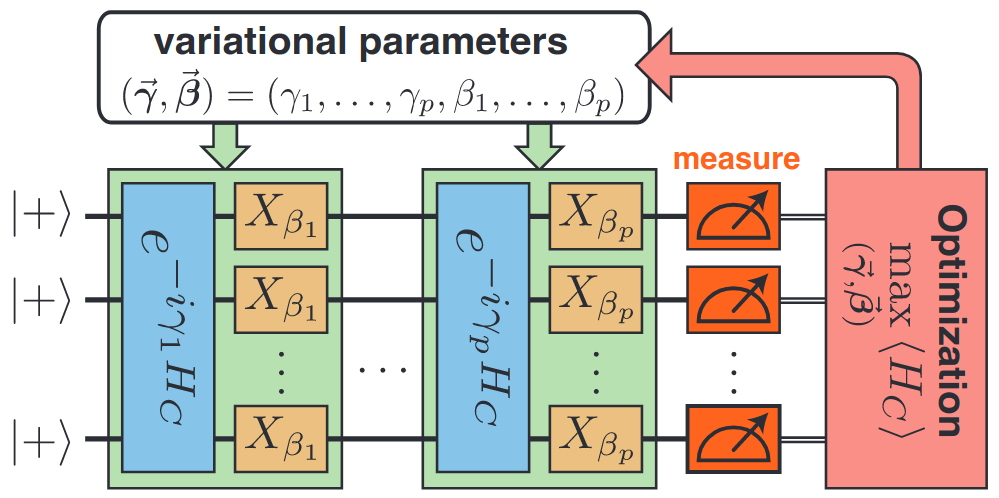
\includegraphics[width=0.6\textwidth]{01-introduction/figs/qaoa.png}
    \caption{Diagram of a $p$-layer QAOA circuit. Starting from the initial state $\ket{+}^{\otimes n}$,the circuit alternates between applying the unitaries $e^{-i \gamma_i \hat{H}_C}$ and $e^{-i \beta_i \hat{H}_M}$ for $i = 1$ to $p$. The final state is measured to estimate the expectation value $\langle \hat{H}_C \rangle$, which is passed to a classical optimizer. This process is repeated until convergence.}
    \vspace{0.3em}
    \small\textit{Source: Adapted from Zhou et al., 2019.~\cite{zhou_quantum_2020}}
    \label{fig:qaoa}
\end{figure}

The Quantum Approximate Optimization Algorithm stands out as one of the most promising approaches for near-term quantum advantage. From a complexity-theoretic perspective, Farhi et al.~\cite{farhi_quantum_2019} argue that sampling from the output distribution of even the shallowest version of QAOA ($p=1$) may already be classically intractable, highlighting its potential as an early demonstration of quantum supremacy.

Beyond this theoretical motivation, QAOA is attractive because of its relatively simple structure and hardware efficiency. Ho and Hsieh~\cite{ho_efficient_2019} introduce a related variational protocol (VQCS), showing that alternating unitaries generated by simple, local Hamiltonians can efficiently prepare non-trivial quantum states and can be implemented on current platforms such as trapped ions and superconducting qubits.

Additionally, QAOA's modularity and variational flexibility make it adaptable to a wide range of applications, including factorization. In particular, Anschuetz et al.~\cite{anschuetz_variational_2018} demonstrate a QAOA-inspired approach to integer factorization, showing that hybrid quantum-classical heuristics can extend QAOA's reach to classically hard problems even on today's noisy devices.

The Quantum Approximate Optimization Algorithm has been extensively investigated since its introduction, leading to a broad landscape of theoretical analyses, practical  implementations, and performance-enhancement techniques. Numerous variants have been proposed, ranging from modified ansatze to parameter initialization heuristics and adaptive layer-scaling procedures. This diversity reflects both the flexibility of the QAOA framework and the complexity of identifying implementations that perform well across different problem instances. This richness also underscores the importance of carefully specifying the algorithmic configuration adopted in any particular study, so that performance comparisons can be made in a meaningful way.